\begin{figure}[h!]
	\centering
	
	
	
	\tikzset{every picture/.style={line width=0.75pt}} %set default line width to 0.75pt        
	
	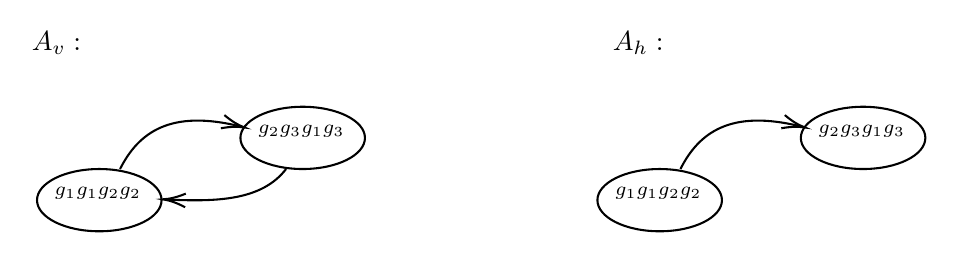
\begin{tikzpicture}[x=0.75pt,y=0.75pt,yscale=-1,xscale=1]
		%uncomment if require: \path (0,300); %set diagram left start at 0, and has height of 300
		
		%Shape: Ellipse [id:dp3480476979550604] 
		\draw   (140,115) .. controls (140,106.72) and (153.43,100) .. (170,100) .. controls (186.57,100) and (200,106.72) .. (200,115) .. controls (200,123.28) and (186.57,130) .. (170,130) .. controls (153.43,130) and (140,123.28) .. (140,115) -- cycle ;
		%Shape: Ellipse [id:dp9456474739758407] 
		\draw   (238,85) .. controls (238,76.72) and (251.43,70) .. (268,70) .. controls (284.57,70) and (298,76.72) .. (298,85) .. controls (298,93.28) and (284.57,100) .. (268,100) .. controls (251.43,100) and (238,93.28) .. (238,85) -- cycle ;
		%Shape: Ellipse [id:dp2502651910875927] 
		\draw   (410,115) .. controls (410,106.72) and (423.43,100) .. (440,100) .. controls (456.57,100) and (470,106.72) .. (470,115) .. controls (470,123.28) and (456.57,130) .. (440,130) .. controls (423.43,130) and (410,123.28) .. (410,115) -- cycle ;
		%Shape: Ellipse [id:dp3792185411216099] 
		\draw   (508,85) .. controls (508,76.72) and (521.43,70) .. (538,70) .. controls (554.57,70) and (568,76.72) .. (568,85) .. controls (568,93.28) and (554.57,100) .. (538,100) .. controls (521.43,100) and (508,93.28) .. (508,85) -- cycle ;
		%Curve Lines [id:da7858938212358939] 
		\draw    (180,100) .. controls (188.87,82.47) and (204.13,70.95) .. (238.42,79.59) ;
		\draw [shift={(240,80)}, rotate = 194.87] [color={rgb, 255:red, 0; green, 0; blue, 0 }  ][line width=0.75]    (10.93,-3.29) .. controls (6.95,-1.4) and (3.31,-0.3) .. (0,0) .. controls (3.31,0.3) and (6.95,1.4) .. (10.93,3.29)   ;
		%Curve Lines [id:da7351349882046846] 
		\draw    (260,100) .. controls (248.11,115.41) and (226.13,115.79) .. (202.43,114.69) ;
		\draw [shift={(200.6,114.6)}, rotate = 2.82] [color={rgb, 255:red, 0; green, 0; blue, 0 }  ][line width=0.75]    (10.93,-3.29) .. controls (6.95,-1.4) and (3.31,-0.3) .. (0,0) .. controls (3.31,0.3) and (6.95,1.4) .. (10.93,3.29)   ;
		%Curve Lines [id:da48287324374825746] 
		\draw    (450,100) .. controls (458.87,82.47) and (474.13,70.95) .. (508.42,79.59) ;
		\draw [shift={(510,80)}, rotate = 194.87] [color={rgb, 255:red, 0; green, 0; blue, 0 }  ][line width=0.75]    (10.93,-3.29) .. controls (6.95,-1.4) and (3.31,-0.3) .. (0,0) .. controls (3.31,0.3) and (6.95,1.4) .. (10.93,3.29)   ;
		
		% Text Node
		\draw (147,107.4) node [anchor=north west][inner sep=0.75pt]  [font=\scriptsize]  {$g_{1} g_{1} g_{2} g_{2}$};
		% Text Node
		\draw (245,77.4) node [anchor=north west][inner sep=0.75pt]  [font=\scriptsize]  {$g_{2} g_{3} g_{1} g_{3}$};
		% Text Node
		\draw (417,107.4) node [anchor=north west][inner sep=0.75pt]  [font=\scriptsize]  {$g_{1} g_{1} g_{2} g_{2}$};
		% Text Node
		\draw (515,77.4) node [anchor=north west][inner sep=0.75pt]  [font=\scriptsize]  {$g_{2} g_{3} g_{1} g_{3}$};
		% Text Node
		\draw (136,32.4) node [anchor=north west][inner sep=0.75pt]    {$A_{v} :$};
		% Text Node
		\draw (416,32.4) node [anchor=north west][inner sep=0.75pt]    {$A_{h} :$};
		
		
	\end{tikzpicture}
\end{figure}